\documentclass[twoside]{book}

% Packages required by doxygen
\usepackage{fixltx2e}
\usepackage{calc}
\usepackage{doxygen}
\usepackage[export]{adjustbox} % also loads graphicx
\usepackage{graphicx}
\usepackage[utf8]{inputenc}
\usepackage{makeidx}
\usepackage{multicol}
\usepackage{multirow}
\PassOptionsToPackage{warn}{textcomp}
\usepackage{textcomp}
\usepackage[nointegrals]{wasysym}
\usepackage[table]{xcolor}

% Font selection
\usepackage[T1]{fontenc}
\usepackage[scaled=.90]{helvet}
\usepackage{courier}
\usepackage{amssymb}
\usepackage{sectsty}
\renewcommand{\familydefault}{\sfdefault}
\allsectionsfont{%
  \fontseries{bc}\selectfont%
  \color{darkgray}%
}
\renewcommand{\DoxyLabelFont}{%
  \fontseries{bc}\selectfont%
  \color{darkgray}%
}
\newcommand{\+}{\discretionary{\mbox{\scriptsize$\hookleftarrow$}}{}{}}

% Page & text layout
\usepackage{geometry}
\geometry{%
  a4paper,%
  top=2.5cm,%
  bottom=2.5cm,%
  left=2.5cm,%
  right=2.5cm%
}
\tolerance=750
\hfuzz=15pt
\hbadness=750
\setlength{\emergencystretch}{15pt}
\setlength{\parindent}{0cm}
\setlength{\parskip}{3ex plus 2ex minus 2ex}
\makeatletter
\renewcommand{\paragraph}{%
  \@startsection{paragraph}{4}{0ex}{-1.0ex}{1.0ex}{%
    \normalfont\normalsize\bfseries\SS@parafont%
  }%
}
\renewcommand{\subparagraph}{%
  \@startsection{subparagraph}{5}{0ex}{-1.0ex}{1.0ex}{%
    \normalfont\normalsize\bfseries\SS@subparafont%
  }%
}
\makeatother

% Headers & footers
\usepackage{fancyhdr}
\pagestyle{fancyplain}
\fancyhead[LE]{\fancyplain{}{\bfseries\thepage}}
\fancyhead[CE]{\fancyplain{}{}}
\fancyhead[RE]{\fancyplain{}{\bfseries\leftmark}}
\fancyhead[LO]{\fancyplain{}{\bfseries\rightmark}}
\fancyhead[CO]{\fancyplain{}{}}
\fancyhead[RO]{\fancyplain{}{\bfseries\thepage}}
\fancyfoot[LE]{\fancyplain{}{}}
\fancyfoot[CE]{\fancyplain{}{}}
\fancyfoot[RE]{\fancyplain{}{\bfseries\scriptsize Generated by Doxygen }}
\fancyfoot[LO]{\fancyplain{}{\bfseries\scriptsize Generated by Doxygen }}
\fancyfoot[CO]{\fancyplain{}{}}
\fancyfoot[RO]{\fancyplain{}{}}
\renewcommand{\footrulewidth}{0.4pt}
\renewcommand{\chaptermark}[1]{%
  \markboth{#1}{}%
}
\renewcommand{\sectionmark}[1]{%
  \markright{\thesection\ #1}%
}

% Indices & bibliography
\usepackage{natbib}
\usepackage[titles]{tocloft}
\setcounter{tocdepth}{3}
\setcounter{secnumdepth}{5}
\makeindex

% Hyperlinks (required, but should be loaded last)
\usepackage{ifpdf}
\ifpdf
  \usepackage[pdftex,pagebackref=true]{hyperref}
\else
  \usepackage[ps2pdf,pagebackref=true]{hyperref}
\fi
\hypersetup{%
  colorlinks=true,%
  linkcolor=blue,%
  citecolor=blue,%
  unicode%
}

% Custom commands
\newcommand{\clearemptydoublepage}{%
  \newpage{\pagestyle{empty}\cleardoublepage}%
}

\usepackage{caption}
\captionsetup{labelsep=space,justification=centering,font={bf},singlelinecheck=off,skip=4pt,position=top}

%===== C O N T E N T S =====

\begin{document}

% Titlepage & ToC
\hypersetup{pageanchor=false,
             bookmarksnumbered=true,
             pdfencoding=unicode
            }
\pagenumbering{roman}
\begin{titlepage}
\vspace*{7cm}
\begin{center}%
{\Large dedup }\\
\vspace*{1cm}
{\large Generated by Doxygen 1.8.11}\\
\end{center}
\end{titlepage}
\clearemptydoublepage
\tableofcontents
\clearemptydoublepage
\pagenumbering{arabic}
\hypersetup{pageanchor=true}

%--- Begin generated contents ---
\chapter{dedup}
\label{md_README}
\hypertarget{md_README}{}
I need a utility to do file level de-\/duplication. This utility will spin through a tree of directories searching for duplicate files (it checks file size and it that matches then sha512) when it finds one (or more) duplicates it hard links them, thus, reducing disc space. I need this because my rsyncs (backups e.\+g. rsync --link-\/dest=...) got out of sync once or twice and now I have a bunch of wasted space; furthermore, dupremove (the btrfs utility that does block level deduplication like say Net\+App) seems to kmalloc all my memory crashing the kernel. This is a bit of a mess right now-\/ it\textquotesingle{}s a hodgepodge of C and C++ (mostly containers) as it is partially an effort to gain as much proficiency with C++ containers as I have with Java containers. The Dia diagram is a bit of a hack too, it\textquotesingle{}s half class diagram half E-\/R (think S\+QL) diagram because R\+D\+B\+M\+Ss are what I\textquotesingle{}m used to, not containers.

Compiler note\+: I\textquotesingle{}m using gcc built from source, I thing it compiles okay on more pedestrian compilers but I\textquotesingle{}m not really checking. I figure by the time this sees the light of day gcc 8.\+whatever will be more mainstream and I was toying with some experimental C++ stuff... C\+O\+L\+L\+E\+C\+T\+\_\+\+G\+CC=gcc C\+O\+L\+L\+E\+C\+T\+\_\+\+L\+T\+O\+\_\+\+W\+R\+A\+P\+P\+ER=/home/tallen/libexec/gcc/x86\+\_\+64-\/pc-\/linux-\/gnu/8.0.\+0/lto-\/wrapper Target\+: x86\+\_\+64-\/pc-\/linux-\/gnu Configured with\+: ../gcc/configure --prefix=/home/tallen --with-\/gmp=/home/tallen --disable-\/multilib Thread model\+: posix gcc version 8.\+0.\+0 20170513 (experimental) (G\+CC) 
\chapter{Class Index}
\section{Class List}
Here are the classes, structs, unions and interfaces with brief descriptions\+:\begin{DoxyCompactList}
\item\contentsline{section}{\hyperlink{class_file}{File} \\*Relevent data about each file in the tree }{\pageref{class_file}}{}
\end{DoxyCompactList}

\chapter{File Index}
\section{File List}
Here is a list of all files with brief descriptions\+:\begin{DoxyCompactList}
\item\contentsline{section}{\hyperlink{_8ycm__extra__conf_8py}{.\+ycm\+\_\+extra\+\_\+conf.\+py} }{\pageref{_8ycm__extra__conf_8py}}{}
\item\contentsline{section}{\hyperlink{dedup_8cc}{dedup.\+cc} }{\pageref{dedup_8cc}}{}
\item\contentsline{section}{\hyperlink{_file_8cc}{File.\+cc} }{\pageref{_file_8cc}}{}
\item\contentsline{section}{\hyperlink{_file_8h}{File.\+h} }{\pageref{_file_8h}}{}
\end{DoxyCompactList}

\chapter{Class Documentation}
\hypertarget{class_file}{}\section{File Class Reference}
\label{class_file}\index{File@{File}}


Relevent data about each file in the tree.  




{\ttfamily \#include $<$File.\+h$>$}

\subsection*{Public Member Functions}
\begin{DoxyCompactItemize}
\item 
\hyperlink{class_file_a068da892ec6464ddf0dcbab2f55962f7}{File} (const std\+::string \&, const std\+::string \&)
\begin{DoxyCompactList}\small\item\em populates various variables \end{DoxyCompactList}\end{DoxyCompactItemize}
\subsection*{Public Attributes}
\begin{DoxyCompactItemize}
\item 
\+\_\+\+\_\+ino\+\_\+t \hyperlink{class_file_a9dadadf265382acd3ac5ca840829b6a6}{inode}
\item 
std\+::string \hyperlink{class_file_ac219294b38d3a3a422ad6ebacb041bb5}{name}
\item 
std\+::string \hyperlink{class_file_a2a3000e706022e1a6e37415ac3984884}{relativepath}
\item 
\hyperlink{_file_8h_a7c56ccac0642bb33c22bec7333682e67}{fsize\+\_\+t} \hyperlink{class_file_aa2ef804960a60130c63406db420e9cdc}{size}
\item 
unsigned char $\ast$ \hyperlink{class_file_ad44605a92eebe23c5738b0d64fdca7e1}{sha} = N\+U\+LL
\item 
bool \hyperlink{class_file_a77110ab18a54c978d72477ee49a0a4cd}{hardlink}
\end{DoxyCompactItemize}
\subsection*{Static Public Attributes}
\begin{DoxyCompactItemize}
\item 
static std\+::map$<$ \+\_\+\+\_\+ino\+\_\+t, \hyperlink{class_file}{File} $\ast$ $>$ \hyperlink{class_file_a32733129d25971738ccba2122b0b91a5}{uk\+\_\+inode}
\item 
static std\+::multimap$<$ \hyperlink{_file_8h_a7c56ccac0642bb33c22bec7333682e67}{fsize\+\_\+t}, \hyperlink{class_file}{File} $\ast$ $>$ \hyperlink{class_file_ab6d7686b65b377692d301aeb171f2788}{cx\+\_\+size}
\end{DoxyCompactItemize}


\subsection{Detailed Description}
Relevent data about each file in the tree. 

This class holds everything related to the files in the the tree. S\+H\+A512\textquotesingle{}s are calculated for files whose file sizes don\textquotesingle{}t make it obvious that they are distinct. 

\subsection{Constructor \& Destructor Documentation}
\index{File@{File}!File@{File}}
\index{File@{File}!File@{File}}
\subsubsection[{\texorpdfstring{File(const std\+::string \&, const std\+::string \&)}{File(const std::string &, const std::string &)}}]{\setlength{\rightskip}{0pt plus 5cm}File\+::\+File (
\begin{DoxyParamCaption}
\item[{const std\+::string \&}]{path, }
\item[{const std\+::string \&}]{filename}
\end{DoxyParamCaption}
)}\hypertarget{class_file_a068da892ec6464ddf0dcbab2f55962f7}{}\label{class_file_a068da892ec6464ddf0dcbab2f55962f7}


populates various variables 

Always populated inode, name, relativepath, and size. adds an entry to the inode and size lookup containers 

\subsection{Member Data Documentation}
\index{File@{File}!cx\+\_\+size@{cx\+\_\+size}}
\index{cx\+\_\+size@{cx\+\_\+size}!File@{File}}
\subsubsection[{\texorpdfstring{cx\+\_\+size}{cx_size}}]{\setlength{\rightskip}{0pt plus 5cm}std\+::multimap$<$ {\bf fsize\+\_\+t}, {\bf File} $\ast$ $>$ File\+::cx\+\_\+size\hspace{0.3cm}{\ttfamily [static]}}\hypertarget{class_file_ab6d7686b65b377692d301aeb171f2788}{}\label{class_file_ab6d7686b65b377692d301aeb171f2788}
\index{File@{File}!hardlink@{hardlink}}
\index{hardlink@{hardlink}!File@{File}}
\subsubsection[{\texorpdfstring{hardlink}{hardlink}}]{\setlength{\rightskip}{0pt plus 5cm}bool File\+::hardlink}\hypertarget{class_file_a77110ab18a54c978d72477ee49a0a4cd}{}\label{class_file_a77110ab18a54c978d72477ee49a0a4cd}
it\textquotesingle{}s alread a hardlink \index{File@{File}!inode@{inode}}
\index{inode@{inode}!File@{File}}
\subsubsection[{\texorpdfstring{inode}{inode}}]{\setlength{\rightskip}{0pt plus 5cm}\+\_\+\+\_\+ino\+\_\+t File\+::inode}\hypertarget{class_file_a9dadadf265382acd3ac5ca840829b6a6}{}\label{class_file_a9dadadf265382acd3ac5ca840829b6a6}
\index{File@{File}!name@{name}}
\index{name@{name}!File@{File}}
\subsubsection[{\texorpdfstring{name}{name}}]{\setlength{\rightskip}{0pt plus 5cm}std\+::string File\+::name}\hypertarget{class_file_ac219294b38d3a3a422ad6ebacb041bb5}{}\label{class_file_ac219294b38d3a3a422ad6ebacb041bb5}
\index{File@{File}!relativepath@{relativepath}}
\index{relativepath@{relativepath}!File@{File}}
\subsubsection[{\texorpdfstring{relativepath}{relativepath}}]{\setlength{\rightskip}{0pt plus 5cm}std\+::string File\+::relativepath}\hypertarget{class_file_a2a3000e706022e1a6e37415ac3984884}{}\label{class_file_a2a3000e706022e1a6e37415ac3984884}
\index{File@{File}!sha@{sha}}
\index{sha@{sha}!File@{File}}
\subsubsection[{\texorpdfstring{sha}{sha}}]{\setlength{\rightskip}{0pt plus 5cm}unsigned char$\ast$ File\+::sha = N\+U\+LL}\hypertarget{class_file_ad44605a92eebe23c5738b0d64fdca7e1}{}\label{class_file_ad44605a92eebe23c5738b0d64fdca7e1}
S\+H\+A512 for the file \index{File@{File}!size@{size}}
\index{size@{size}!File@{File}}
\subsubsection[{\texorpdfstring{size}{size}}]{\setlength{\rightskip}{0pt plus 5cm}{\bf fsize\+\_\+t} File\+::size}\hypertarget{class_file_aa2ef804960a60130c63406db420e9cdc}{}\label{class_file_aa2ef804960a60130c63406db420e9cdc}
\index{File@{File}!uk\+\_\+inode@{uk\+\_\+inode}}
\index{uk\+\_\+inode@{uk\+\_\+inode}!File@{File}}
\subsubsection[{\texorpdfstring{uk\+\_\+inode}{uk_inode}}]{\setlength{\rightskip}{0pt plus 5cm}std\+::map$<$ \+\_\+\+\_\+ino\+\_\+t, {\bf File} $\ast$ $>$ File\+::uk\+\_\+inode\hspace{0.3cm}{\ttfamily [static]}}\hypertarget{class_file_a32733129d25971738ccba2122b0b91a5}{}\label{class_file_a32733129d25971738ccba2122b0b91a5}


The documentation for this class was generated from the following files\+:\begin{DoxyCompactItemize}
\item 
\hyperlink{_file_8h}{File.\+h}\item 
\hyperlink{_file_8cc}{File.\+cc}\end{DoxyCompactItemize}

\chapter{File Documentation}
\hypertarget{_8ycm__extra__conf_8py}{}\section{.ycm\+\_\+extra\+\_\+conf.\+py File Reference}
\label{_8ycm__extra__conf_8py}\index{.\+ycm\+\_\+extra\+\_\+conf.\+py@{.\+ycm\+\_\+extra\+\_\+conf.\+py}}

\hypertarget{dedup_8cc}{}\section{dedup.\+cc File Reference}
\label{dedup_8cc}\index{dedup.\+cc@{dedup.\+cc}}
{\ttfamily \#include $<$string$>$}\\*
{\ttfamily \#include \char`\"{}File.\+h\char`\"{}}\\*
Include dependency graph for dedup.\+cc\+:
\nopagebreak
\begin{figure}[H]
\begin{center}
\leavevmode
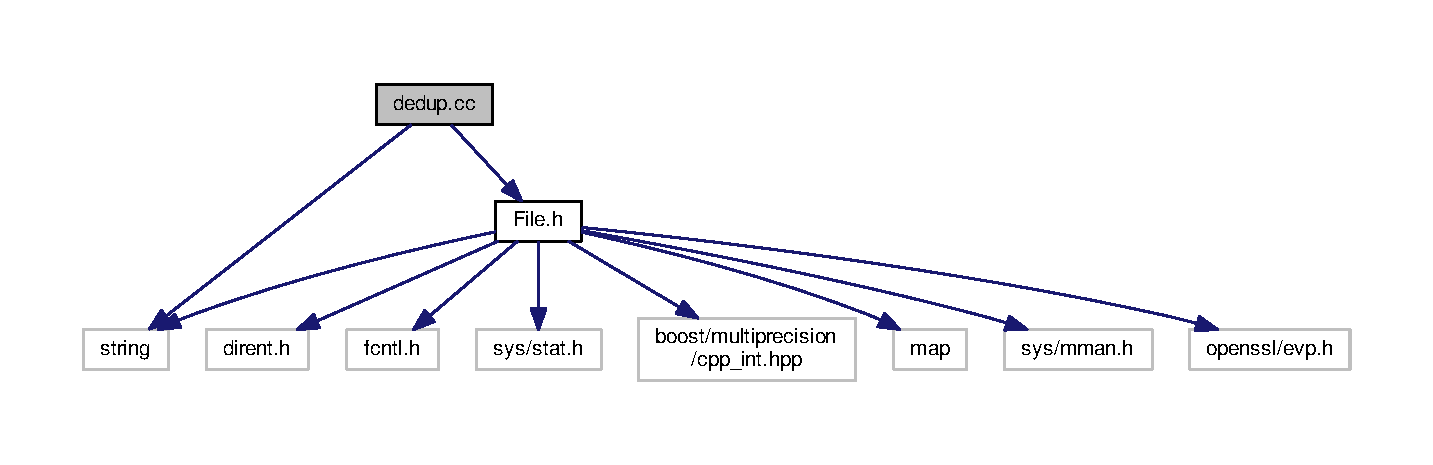
\includegraphics[width=350pt]{dedup_8cc__incl}
\end{center}
\end{figure}
\subsection*{Functions}
\begin{DoxyCompactItemize}
\item 
void \hyperlink{dedup_8cc_ad478736cd4716b31b43f951ba4214958}{statdir} (const std\+::string \&path)
\item 
void \hyperlink{dedup_8cc_a53a8eac96bcf45d21220d6b21776964d}{printsha} (unsigned int $\ast$sha)
\item 
int \hyperlink{dedup_8cc_a1c03069360f1f90a556eb537e0ff8a72}{main} (int argv, char $\ast$$\ast$argc)
\end{DoxyCompactItemize}


\subsection{Function Documentation}
\index{dedup.\+cc@{dedup.\+cc}!main@{main}}
\index{main@{main}!dedup.\+cc@{dedup.\+cc}}
\subsubsection[{\texorpdfstring{main(int argv, char $\ast$$\ast$argc)}{main(int argv, char **argc)}}]{\setlength{\rightskip}{0pt plus 5cm}int main (
\begin{DoxyParamCaption}
\item[{int}]{argv, }
\item[{char $\ast$$\ast$}]{argc}
\end{DoxyParamCaption}
)}\hypertarget{dedup_8cc_a1c03069360f1f90a556eb537e0ff8a72}{}\label{dedup_8cc_a1c03069360f1f90a556eb537e0ff8a72}
\index{dedup.\+cc@{dedup.\+cc}!printsha@{printsha}}
\index{printsha@{printsha}!dedup.\+cc@{dedup.\+cc}}
\subsubsection[{\texorpdfstring{printsha(unsigned int $\ast$sha)}{printsha(unsigned int *sha)}}]{\setlength{\rightskip}{0pt plus 5cm}void printsha (
\begin{DoxyParamCaption}
\item[{unsigned int $\ast$}]{sha}
\end{DoxyParamCaption}
)}\hypertarget{dedup_8cc_a53a8eac96bcf45d21220d6b21776964d}{}\label{dedup_8cc_a53a8eac96bcf45d21220d6b21776964d}
\index{dedup.\+cc@{dedup.\+cc}!statdir@{statdir}}
\index{statdir@{statdir}!dedup.\+cc@{dedup.\+cc}}
\subsubsection[{\texorpdfstring{statdir(const std\+::string \&path)}{statdir(const std::string &path)}}]{\setlength{\rightskip}{0pt plus 5cm}void statdir (
\begin{DoxyParamCaption}
\item[{const std\+::string \&}]{path}
\end{DoxyParamCaption}
)}\hypertarget{dedup_8cc_ad478736cd4716b31b43f951ba4214958}{}\label{dedup_8cc_ad478736cd4716b31b43f951ba4214958}

\hypertarget{_file_8cc}{}\section{File.\+cc File Reference}
\label{_file_8cc}\index{File.\+cc@{File.\+cc}}
{\ttfamily \#include \char`\"{}File.\+h\char`\"{}}\\*
Include dependency graph for File.\+cc\+:
\nopagebreak
\begin{figure}[H]
\begin{center}
\leavevmode
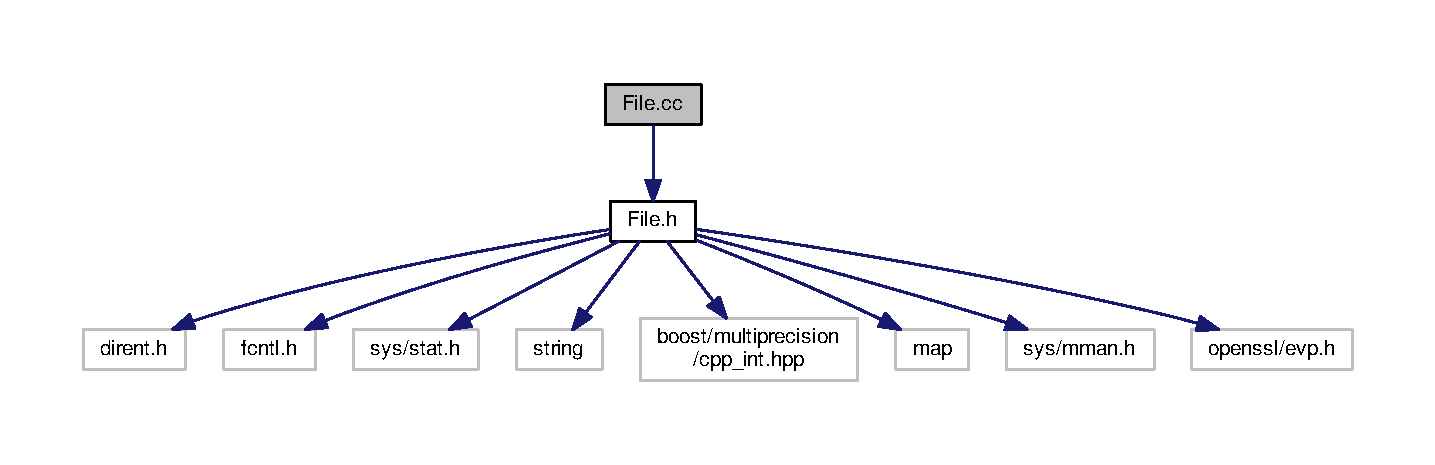
\includegraphics[width=350pt]{_file_8cc__incl}
\end{center}
\end{figure}

\hypertarget{_file_8h}{}\section{File.\+h File Reference}
\label{_file_8h}\index{File.\+h@{File.\+h}}
{\ttfamily \#include $<$dirent.\+h$>$}\\*
{\ttfamily \#include $<$fcntl.\+h$>$}\\*
{\ttfamily \#include $<$sys/stat.\+h$>$}\\*
{\ttfamily \#include $<$string$>$}\\*
{\ttfamily \#include $<$boost/multiprecision/cpp\+\_\+int.\+hpp$>$}\\*
{\ttfamily \#include $<$map$>$}\\*
{\ttfamily \#include $<$sys/mman.\+h$>$}\\*
{\ttfamily \#include $<$openssl/evp.\+h$>$}\\*
Include dependency graph for File.\+h\+:
\nopagebreak
\begin{figure}[H]
\begin{center}
\leavevmode
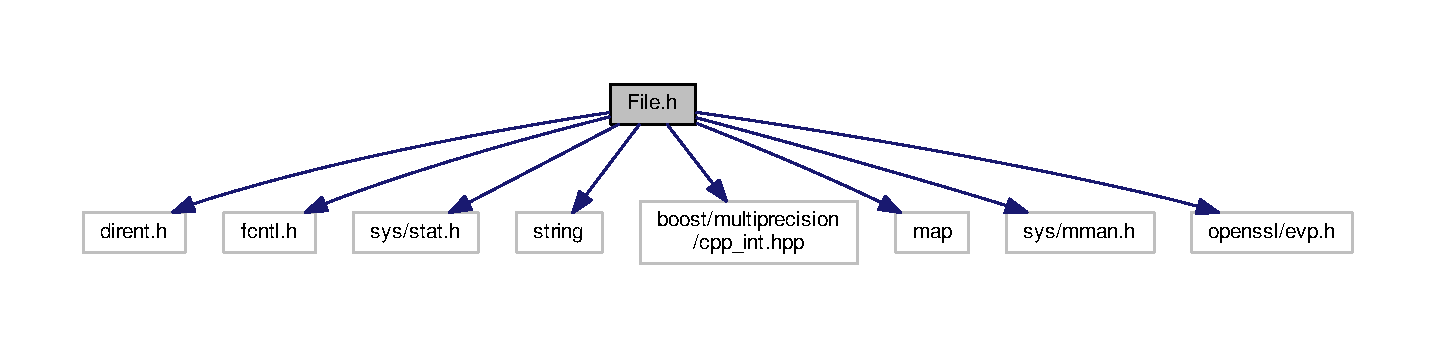
\includegraphics[width=350pt]{_file_8h__incl}
\end{center}
\end{figure}
This graph shows which files directly or indirectly include this file\+:
\nopagebreak
\begin{figure}[H]
\begin{center}
\leavevmode
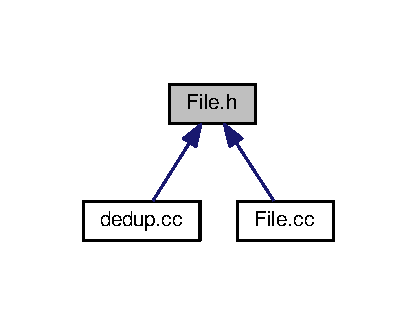
\includegraphics[width=200pt]{_file_8h__dep__incl}
\end{center}
\end{figure}
\subsection*{Classes}
\begin{DoxyCompactItemize}
\item 
class \hyperlink{class_file}{File}
\begin{DoxyCompactList}\small\item\em Relevent data about each file in the tree. \end{DoxyCompactList}\end{DoxyCompactItemize}
\subsection*{Typedefs}
\begin{DoxyCompactItemize}
\item 
typedef off\+\_\+t \hyperlink{_file_8h_a7c56ccac0642bb33c22bec7333682e67}{fsize\+\_\+t}
\end{DoxyCompactItemize}


\subsection{Typedef Documentation}
\index{File.\+h@{File.\+h}!fsize\+\_\+t@{fsize\+\_\+t}}
\index{fsize\+\_\+t@{fsize\+\_\+t}!File.\+h@{File.\+h}}
\subsubsection[{\texorpdfstring{fsize\+\_\+t}{fsize_t}}]{\setlength{\rightskip}{0pt plus 5cm}typedef off\+\_\+t {\bf fsize\+\_\+t}}\hypertarget{_file_8h_a7c56ccac0642bb33c22bec7333682e67}{}\label{_file_8h_a7c56ccac0642bb33c22bec7333682e67}

\hypertarget{_r_e_a_d_m_e_8md}{}\section{R\+E\+A\+D\+M\+E.\+md File Reference}
\label{_r_e_a_d_m_e_8md}\index{R\+E\+A\+D\+M\+E.\+md@{R\+E\+A\+D\+M\+E.\+md}}

%--- End generated contents ---

% Index
\backmatter
\newpage
\phantomsection
\clearemptydoublepage
\addcontentsline{toc}{chapter}{Index}
\printindex

\end{document}
